% Paper template for TAR 2022
% (C) 2014 Jan Šnajder, Goran Glavaš, Domagoj Alagić, Mladen Karan
% TakeLab, FER

\documentclass[10pt, a4paper]{article}

\usepackage{tar2023}

\usepackage[utf8]{inputenc}
\usepackage[pdftex]{graphicx}
\usepackage{booktabs}
\usepackage{amsmath}
\usepackage{amssymb}

\title{Well, some find it funny: Exploring alternative methods of combining Humicroedit annotator scores}

\name{Dorijan Cirkveni} 

\address{
University of Zagreb, Faculty of Electrical Engineering and Computing\\
Unska 3, 10000 Zagreb, Croatia\\ 
\texttt{autor1@xxx.hr}, \texttt{\{autor2,autor3\}@zz.com}\\
}
          
         
\abstract{
Humor is an inherently subjective matter, as can be seen in the Humicroedit dataset's annotator grades which diverge greatly for higher averages, which this paper suggests might require an annotation analysis method different than those traditionally used on high-agreement datasets. In order to achieve a more evenly distributed labeling system, this paper uses a weighted mean and a variety of methods to determine the ideal set of weights, and then compares performance on dataset with the regular mean.
}

\begin{document}

\maketitleabstract

\section{Introduction}

Artificial intelligence has been making major strides recently both in terms of development and practical usage, especially with the advent of LLMs such as ChatGPT as well as stable diffusion models such as Midjourney. However, certain tasks still remain outside its grasp. 

One such task is the detection, analysis, and generation of humor, a task that continues to elude the methods used. And unlike humor recognition (Khodak et al., 2017; Davidov et al., 2010; Barbieri and Saggion, 2014; Reyes et al., 2012; Cattle and Ma, 2018; Bertero and Fung, 2016; Yang et al., 2015), humor generation using artificial intelligence has proven especially tasking. One obstacle in this line of research is the scarcity of public datasets, and even greater scarcity - if not outright absence - of topic-appropriate public datasets.

One large problem in this field of study is bias, because humor is as subjective as it is complex which makes it significantly challenging to tackle from a natural language analysis/synthesis standpoint.

There are two common approaches to this problem in terms of reducing domain size and therefore annotator bias, one being to focus on a specific domain (TODO: insert citations) and the other being to focus on a specific research topic.

\subsection{Humicroedit}
\label{sec:HME}

The underlying paper of this paper, \textit{“President Vows to Cut Taxes Hair”:
Dataset and Analysis of Creative Text Editing for Humorous Headlines} (Hossain et al., 2019), provides one dataset that is an example of the latter. A lot of care was put into 

\section{Related Work}





\section{Humicroedit data properties}
As mentioned in~\ref{sec:HME}, Humicroedit was designed with an intention of . However, as noted in the paper, despite the writers' effort of carefully qualifying annotators, their perception of headlines in regards of humor present was influenced by their knowledge, preferences, 
Despite us carefully qualifying annotators, their
knowledge, preferences, bias and stance towards information presented in headlines influence whether they perceive a potentially funny
headline as humorous, offensive, confusing, etc.

\begin{figure}
\begin{center}
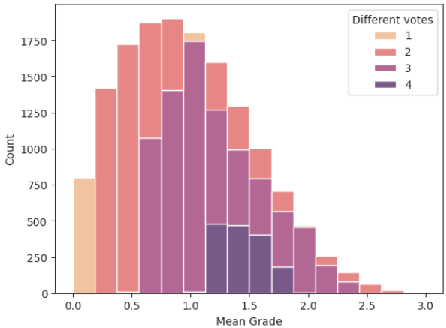
\includegraphics[width=\columnwidth]{vote distribution.pdf}
\caption{Distribution of votes for entire dataset.}
\label{fig:figure1}
\end{center}
\end{figure}

This bias is best seen in the annotator vote distribution, as lower mean scores are closer to unanimous than higher mean scores (as well as more common) as seen in Figure~\ref{fig:figure1}.


Annotator bias presents itself in topic frequency, as seen by one topic that appears in dataset entries more often than any other, as seen in Figure~\ref{fig:figure2} at 39 percent of the total dataset size.

\begin{figure}
\begin{center}
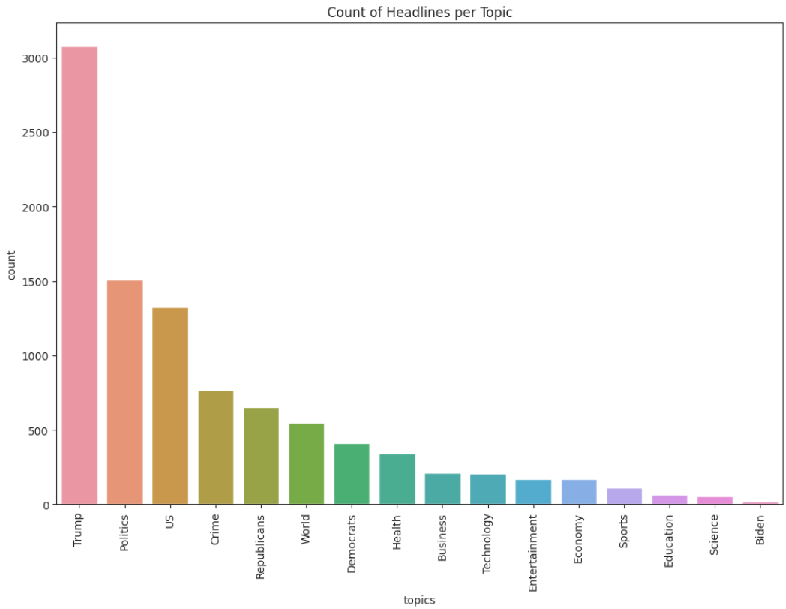
\includegraphics[width=\columnwidth]{topics_disproportion.pdf}
\caption{As we can see on this chart, a disproportionate amount of headline edits has been written on the topic of Donald J. Trump, a notable and controversial media personality and then-incumbent (45th) president of the United States of America.}
\label{fig:figure2}
\end{center}
\end{figure}

However, it does not appear that this topic has a notable difference 
\begin{figure}
\begin{center}
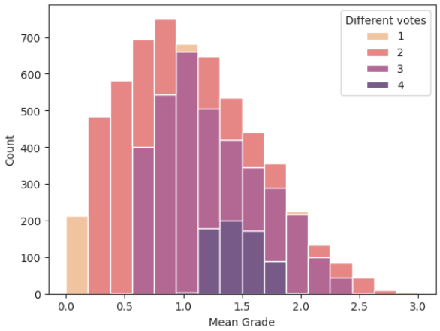
\includegraphics[width=\columnwidth]{t vote distribution.pdf}
\caption{Distribution of votes for most common topic.}
\label{fig:figure1}
\end{center}
\end{figure}



\section{Distribution measurement methods}
In order to effectively choose our weights, visual confirmation will not be a sufficient measure.
In this paper we shall use 4 different methods of determining how even is the label distribution: the Chi-Square uniformity test, the Kolmogorov-Smirnov uniformity test, the Cramér-von Mises uniformity test, and a custom uniformity test developed specifically for this purpose.
\subsection{Custom uniformity test}
The custom uniformity test is based on the method we used to display unevenly wide histogram bars:

\begin{enumerate}
\item n is the number of unique values, and the number of bars. $x_i$ is value of unique value i, and $y_i$ is its frequency.

\item Set up limits between unique values to their arithmetic mean,

\begin{equation}\label{eq:bars}
lim_i = (x_i + x_i+1)/2, i>0,i<n
\end{equation}

\item Set up beginning and end limits in a way that first and last bars are centered on their values
\begin{equation}\label{eq:lim_0}
lim_0 = x_0*2 - lim_1
\end{equation}
\begin{equation}\label{eq:lim_n}
lim_n = x_n*2 - lim_n-1
\end{equation}

\item Calculate densities of data for each bar:
\begin{equation}\label{eq:lim_n}
d_i = y_i/(lim_i+1 - lim_i) i>=0,i<n
\end{equation}

\item Calculate reference density (for perfect set):
\begin{equation}\label{eq:lim_n}
d_{total} = y/(lim_n - lim_0)
\end{equation}

\item Apply weighted square mean error:
\begin{equation}\label{eq:lim_n}
sme = \sum_{i=1}^n (lim_i+1 - lim_i)*(d_i-d_{total})^2
\end{equation}


\item Divide result by reference density square:
\begin{equation}\label{eq:lim_n}
sme_{adjusted} = sme/(lim_i+1 - lim_i)*d_{total}^2
\end{equation}
\end{enumerate}

\subsection{Unweighted arithmetic mean}
First, we will determine the base distribution values by testing them on the provided labels, and the result of this are visible in Table 1.

Unfort
\begin{table}
\caption{Using methods on standard mean}
\label{tab:narrow-table}
\begin{center}
\begin{tabular}{ll}
\toprule
Method & Result \\
\midrule
Custom Uniformity & 4.350 \\
Chi Square Uniformity & 5114.936 \\
Kolmogorov-Smirnov Uniformity & 0.0 (error) \\
Cramér-von Mises Uniformity & 1056.477 \\
\bottomrule
\end{tabular}
\end{center}
\end{table}

\section{Figures and tables}

\subsection{Figures}

Here is an example on how to include figures in the paper. Figures are included in \LaTeX{} code immediately \textit{after} the text in which these figures are referenced. Allow \LaTeX{} to place the figure where it believes is best (usually on top of the page of at the position where you would not place the figure). Figures are referenced as follows: ``Figure shows \dots''. Use tilde (\verb.~.) to prevent separation between the word ``Figure'' and its enumeration. 

\subsection{Tables}

There are two types of tables: narrow tables that fit into one column and a wide table that spreads over both columns.

\subsubsection{Narrow tables}

Table~\ref{tab:narrow-table} is an example of a narrow table. Do not use vertical lines in tables -- vertical tables have no effect and they make tables visually less attractive. We recommend using \textit{booktabs} package for nicer tables.

\begin{table}
\caption{This is the caption of the table. Table captions should be placed \textit{above} the table.}
\label{tab:narrow-table}
\begin{center}
\begin{tabular}{ll}
\toprule
Heading1 & Heading2 \\
\midrule
One & First row text \\
Two   & Second row text \\
Three   & Third row text \\
      & Fourth row text \\
\bottomrule
\end{tabular}
\end{center}
\end{table}

\subsection{Wide tables}

Table~\ref{tab:wide-table} is an example of a wide table that spreads across both columns. The same can be done for wide figures that should spread across the whole width of the page. 

\begin{table*}
\caption{Wide-table caption}
\label{tab:wide-table}
\begin{center}
\begin{tabular}{llr}
\toprule
Heading1 & Heading2 & Heading3\\
\midrule
A & A very long text, longer that the width of a single column & $128$\\
B & A very long text, longer that the width of a single column & $3123$\\
C & A very long text, longer that the width of a single column & $-32$\\
\bottomrule
\end{tabular}
\end{center}
\end{table*}

\section{Math expressions and formulas}



\section{Referencing literature}

References to other publications should be written in brackets with the last name of the first author and the year of publication, e.g., \citep{chomsky-73}.  Multiple references are written in sequence, one after another, separated by semicolon and without whitespaces in between, e.g., \citep{chomsky-73,chave-64,feigl-58}. References are typically written at the end of the sentence and necessarily before the sentence punctuation.

If the publication is authored by more than one author, only the name of the first author is written, after which abbreviation \emph{et al.}, meaning \emph{et alia}, i.e.,~and others is written as in \citep{johnson-etc}. If the publication is authored by only two authors, then the last names of both authors are written \citep{johnson-howells}.

If the name of the author is incorporated into the text of the sentence, it should not be in the brackets (only the year should be there). E.g.,~``\citet{chomsky-73}
suggested that \dots''. The difference is whether you reference the publication or the author who wrote it. 

The list of all literature references is given alphabetically at the end of the paper. The form of the reference depends on the type of the bibliographic unit: conference papers,
\citep{chave-64}, books \citep{butcher-81}, journal articles
\citep{howells-51}, doctoral dissertations \citep{croft-78}, and book chapters \citep{feigl-58}. 

All of this is automatically produced when using BibTeX. Insert all the BibTeX entries into the file \texttt{tar2023.bib}, and then reference them via their symbolic names.

\section{Conclusion}

Conclusion is the last enumerated section of the paper. It should not exceed half of a column and is typically split into 2--3 paragraphs. No new information should be presented in the conclusion; this section only summarizes and concludes the paper.

\section*{Acknowledgements}

If suitable, you can include the \textit{Acknowledgements} section before inserting the literature references  in order to thank those who helped you in any way to deliver the paper, but are not co-authors of the paper.

\bibliographystyle{tar2023}
\bibliography{tar2023} 

\end{document}

